\section{Methoden und Implementierung} % (fold)
\label{sec:methoden_und_implementierung}

  \subsection{Programmstruktur} % (fold)
  \label{sub:strukturen}

    Das von uns erstellte Programm dient der numerischen Approximation von Lösungen des $n$-Körper-Problems für gegebene Anfangswerte.
    Um die Auswertung von Ergebnissen zu vereinfachen und intuitiver zu gestalten, implementierten wir neben den Integratoren eine graphische Ausgabe, eine einfache Form der Eingabe und diverse Möglichkeiten, um zwischen verschiedenen Einstellungen und Integratoren zur Laufzeit des Programmes zu wechseln.

    Bei der Ausgabe handelt es sich um eine perspektivische Projektion des betrachteten Raums auf den Bildschirm einer virtuellen Kamera.
    Position und Ausrichtung der Kamera lassen sich durch Mausinteraktionen beliebig einstellen.
    Zur Orientierung und Größeneinschätzung wird das Gitter eines Würfels mit Kantenlänge $1$ im Koordinatenursprung gezeigt.
    Die Punktmassen werden durch Kugeln dargestellt, deren Radien entsprechend ihrer Masse und ihres Abstandes zur Kamera skaliert werden.
    % Bananen waren keine gute Idee.
    Um die zurückgelegten Kurven der Partikel zu visualisieren, speicherten wir eine feste Anzahl von Bahnpunkten und verbanden diese durch Strecken.
    Das Tracken der Bahnpunkte erfolgte nicht nach jedem Zeitschritt, sondern wurde durch ein Kriterium festgelegt, welches sicher stellte, dass nur Punkte festgehalten wurden, die eine signifikante Richtungsänderung der Kurve hervorriefen.
    In Abbildung \ref{fig:program_example} werden die angegebenen Methoden noch einmal anhand eines Beispiels demonstriert.

    \begin{figure}[h]
      \center
      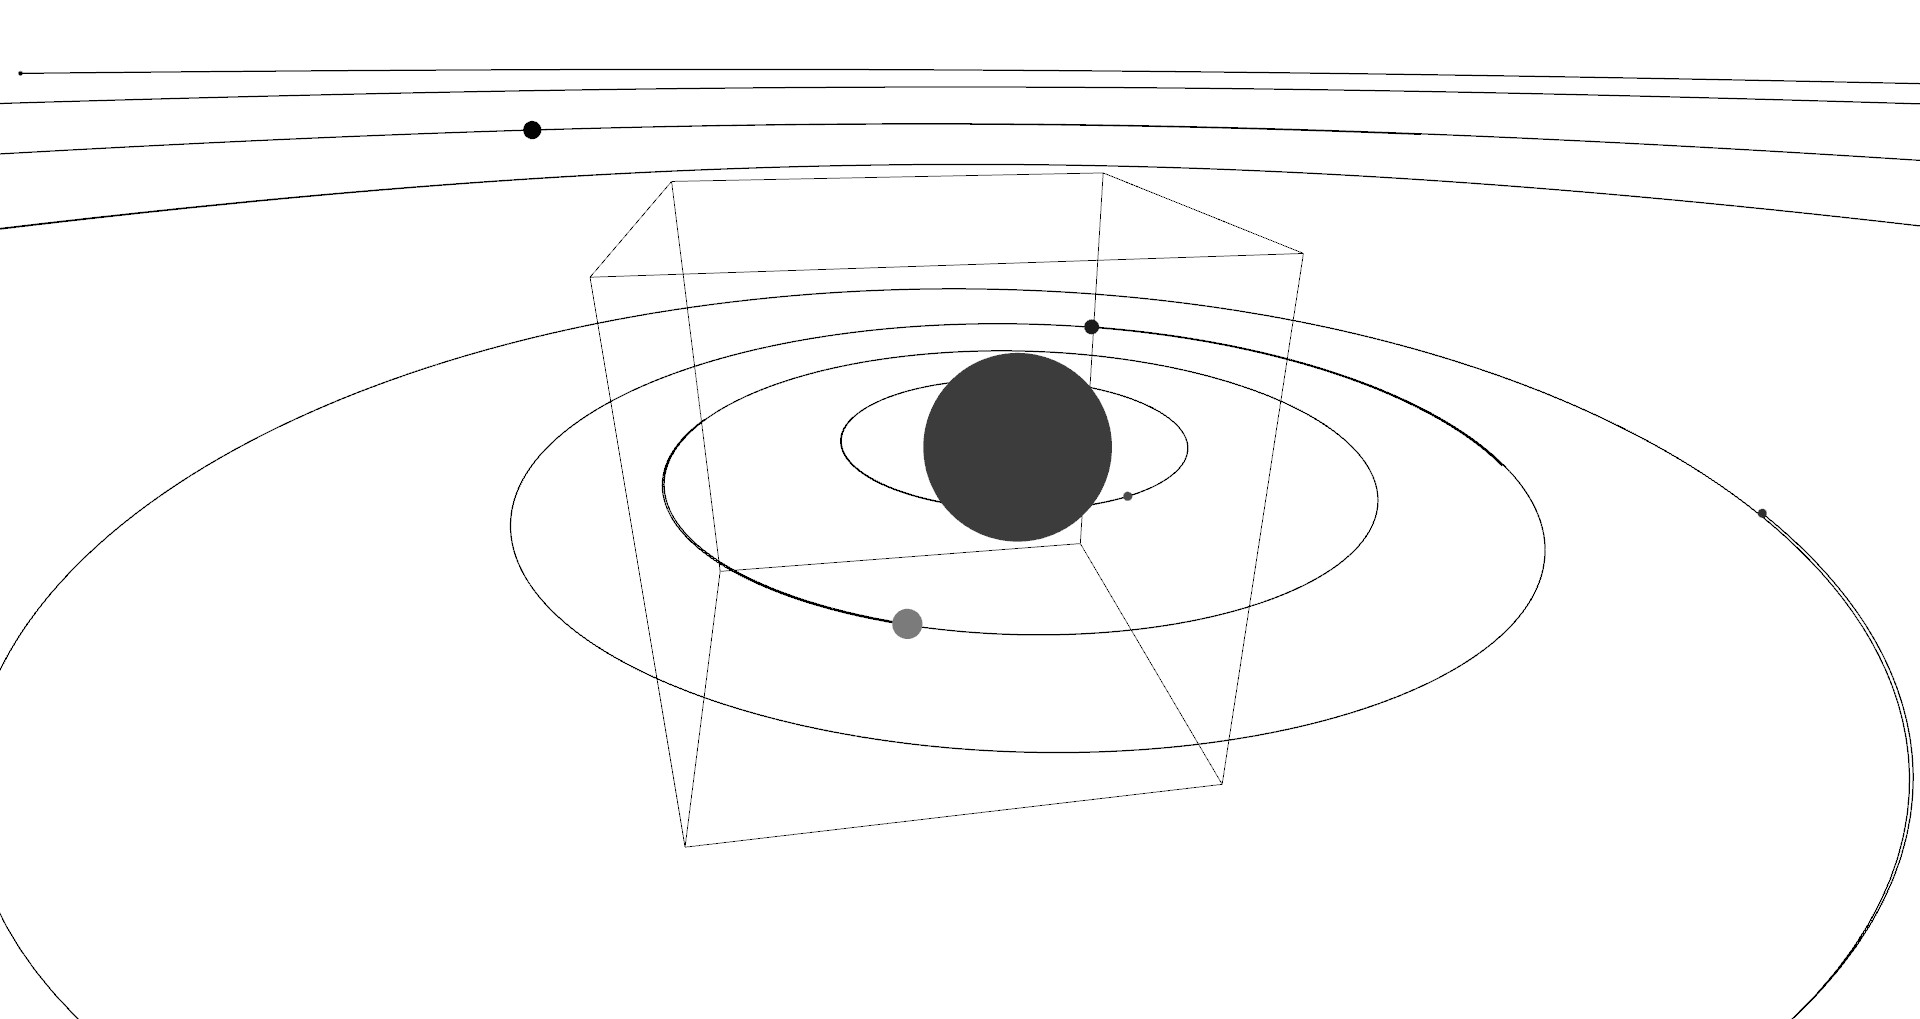
\includegraphics[width=0.95\textwidth]{pictures/program_example.jpg}
      \caption{Die Abbildung zeigt die Ausgabe des Programmes unter Verwendung des Sonnensystems als Beispielszenario. Zu erkennen sind unterschiedlich große Punktmassen und deren Bahnkurven. Das gezeigte Würfelgitter besitzt eine Kantenlänge von $1$.}
      \label{fig:program_example}
    \end{figure}

    Um die noch folgenden Integratoren zu verstehen und implementieren zu können, muss im Vorfeld über eine feste Datenstruktur, welche beschreibt, wie Positionen, Geschwindigkeiten und Massen der einzelnen Partikel zu speichern sind, entschieden werden.
    Zwei typische Varianten für eine solche Datenstruktur werden mit AOS (Array-of-Structure) und SOA (Structure-of-Array) bezeichnet.
    Im Folgenden sind für diese beiden Fälle einfache C++-Quelltexte angegeben.
    In beiden Fällen werden auf die C++-Standardbibliothek und die Bibliothek Eigen zugegriffen.
    Im Programm legten wir uns auf die AOS-Datenstruktur fest, da sie intuitiver im Umgang ist.
    \medskip
    \begin{tcolorbox}[colframe=black,colbacktitle=white,coltitle=black, attach boxed title to top center={yshift=-2mm},enhanced, titlerule=0.1pt, boxrule=0.5pt, arc=5pt,title=Quelltext:\quad SOA-Partikelsystem-Datenstruktur, breakable]
      \lstinputlisting[style=std,language=c++]{code/particle_system_soa.h}
    \end{tcolorbox}
    % \medskip

    % \medskip
    \begin{tcolorbox}[colframe=black,colbacktitle=white,coltitle=black, attach boxed title to top center={yshift=-2mm},enhanced, titlerule=0.1pt, boxrule=0.5pt, arc=5pt,title=Quelltext:\quad AOS-Partikelsystem-Datenstruktur, breakable]
      \lstinputlisting[style=std,language=c++]{code/particle_system_aos.h}
    \end{tcolorbox}

  % subsection strukturen (end)

  \subsection{Berechnung der Beschleunigung} % (fold)
  \label{sub:berechnung_der_beschleunigung}

    Die Berechnung der Beschleunigung kann direkt mithilfe der Gleichung aus Abschnitt \ref{sub:das_n_koerper_problem} erfolgen, indem für ein gegebenen Index $i\in\setNatural$ mit $i\leq n$ über alle anderen Partikel iteriert wird.
    \[
      a_i(r_1,\ldots,r_n) = \sum_{{j=1,\ j\neq i}}^n \gamma m_j \frac{r_j-r_i}{\norm{r_j-r_i}^3}
    \]
    Um jedoch numerische Singularitäten zu vermeiden, führten wir einen Parameter $\varepsilon\in\setReal^+$ ein, der sicherstellt, dass der Nenner des Bruches stets größer Null ist.
    Die leicht variierte Beschleunigung $\tilde{a}$ kann für alle $i\in\setNatural$ mit $i\leq n$ mit der folgenden Gleichung berechnet werden.
    \[
      \tilde{a}_i(r_1,\ldots,r_n)\define \sum_{{j=1,\ j\neq i}}^n \gamma m_j \frac{r_j-r_i}{\norm{r_j-r_i}^3 + \varepsilon}
    \]
    Zu beachten ist, dass durch die Einführung von $\varepsilon$ die Beschleunigung, die eine Punktmasse durch sich selbst erfährt, jetzt definiert und stets Null ist.
    \[
      \tilde{a}_i(r_1,\ldots,r_n) = \sum_{{j=1}}^n \gamma m_j \frac{r_j-r_i}{\norm{r_j-r_i}^3 + \varepsilon}
    \]
    Aus diesem Grund kann eine if-Abfrage für $i\neq j$ im Quelltext entfallen.
    Dies steigert das Optimierungspotential des Compilers und damit auch die resultierende Effizienz und Berechnungsgeschwindigkeit.
    Eine beispielhafte Implementierung in C++ ist im folgenden Quellcode gezeigt.

    \medskip
    \begin{tcolorbox}[colframe=black,colbacktitle=white,coltitle=black, attach boxed title to top center={yshift=-2mm},enhanced, titlerule=0.1pt, boxrule=0.5pt, arc=5pt,title=Quelltext:\quad Partikel-Beschleunigung, breakable]
      \lstinputlisting[style=std,language=c++]{code/particle_acceleration.cc}
    \end{tcolorbox}

  % subsection berechnung_der_beschleunigung (end)

  \subsection{Integratoren} % (fold)
  \label{sub:integratoren}

    Integratoren oder auch numerische Integratoren bezeichnen in der numerischen Mathematik Algorithmen, die entweder den Wert eines bestimmten Integrals oder die Lösung einer Differentialgleichung numerisch approximieren.
    Wir möchten uns hier auf die numerische Lösung von gewöhnlichen Differentialgleichungen beschränken.
    Integratoren werden immer dann verwendet, wenn analytische Lösungen nicht existieren oder zu kompliziert sind.
    In diesen Fällen reicht es aus, genäherte Lösungen mit beliebig kleinem Fehler zu bestimmen.

    Gerade beim $n$-Körper-Problem für $n\geq 3$ ist es demnach notwendig Integratoren zu verwenden, da allgemeine geschlossene Lösungen nicht existieren.
    Alle der hier verwendeten Integratoren lösen gewöhnliche Differentialgleichungssysteme erster Ordnung.
    Allerdings lässt sich das $n$-Körper-Problem wie in Abschnitt $\ref{sub:das_n_koerper_problem}$ gezeigt, in ein solches System überführen.

    Integratoren lassen sich nach ihrer Stabilität oder Robustheit, ihrer Genauigkeit und ihrer Geschwindigkeit einordnen.
    Die Geschwindigkeit ist durch eine einfache Zeitmessung bestimmbar.
    Um die Stabilität eines Integrators einzuschätzen, betrachten wir die Gesamtenergie des Systems, welche nach dem Energieerhaltungssatz konstant bleiben muss.
    Die Simulation eines analytisch lösbaren Problems, wie zum Beispiel des Zweikörperproblems, macht es zudem möglich die Genauigkeit eines Integrators zu bewerten.

    In den folgenden Abschnitten betrachten wir einige typische Integratoren, implementieren diese und schätzen sie nach den genannten Kriterien ein.
    Für $k\in\setNatural$ nennen wir $t_k\in\setReal^+$ den $k$.~Zeitpunkt mit der Bedingung $t_k < t_{k+1}$ für alle $k\in\setNatural$.
    Zudem nennen wir den $\Delta t \define t_{k+1}-t_k$ den Zeitschritt für äquidistante Zeitdiskretisierungen.
    Des Weiteren definieren wir $p_k$ als die numerische Approximation des gewählten Integrators von $p(t_k)$ für alle $k\in\setNatural$.

  % subsection integratoren (end)

  \subsection{Explizites Euler-Verfahren} % (fold)
  \label{sub:euler_verfahren}

    Das explizite Euler-Verfahren ist eines der simpelsten und intuitivsten Verfahren zur Approximation von gewöhnlichen Differentialgleichungen erster Ordnung.
    Dieses einfache Verfahren nähert die Zeitableitung in der Differentialgleichung durch den diskreten rechtsseitigen Differenzenquotient.
    Gemäß unserer Notation aus Abschnitt \ref{sub:das_n_koerper_problem} kann der explizite Euler-Algorithmus für alle $k \in \setNatural$ mit gegebenen Anfangswerten $p_1$ wie folgt aufgeschrieben werden.
    \[
      p_{k+1} = p_k + \Delta t \cdot f(p_k)
    \]
    Eine äquivalente Formulierung für die Kurven des Konfigurationsraumes ist im folgenden Gleichungssystem gegeben.
    \[
      \begin{pmatrix}
        r_{k+1} \\ v_{k+1}
      \end{pmatrix}
      \define
      \begin{pmatrix}
        r_k \\ v_k
      \end{pmatrix}
      + \Delta t \cdot
      \begin{pmatrix}
        v_k \\ a(r_k)
      \end{pmatrix}
    \]
    Das explizite Euler-Verfahren konvergiert in erster Ordnung mit dem Zeitschritt $\Delta t$.
    Im Allgemeinen erhält es nicht die Energie des betrachteten Systems.
    \medskip
    \begin{tcolorbox}[colframe=black,colbacktitle=white,coltitle=black, attach boxed title to top center={yshift=-2mm},enhanced, titlerule=0.1pt, boxrule=0.5pt, arc=5pt,title=Quelltext:\quad Expliziter Euler-Integrator, breakable]
      \lstinputlisting[style=std,language=c++]{code/euler_integrator.cc}
    \end{tcolorbox}

  % subsection euler_verfahren (end)

  \subsection{Symplektisches Euler-Verfahren} % (fold)
  \label{sub:symplektisches_euler_verfahren}

    Verfahren wie der explizite Euler, die keine Energieerhaltung aufweisen, neigen dazu nummerische Fahler in jedem Schritt aufzusummieren, wodurch die numerische Lösung mit der Zeit immer weiter von der analytischen weg driftet.
    Ein Lösungsansatz für dieses Problem sind symplektische Verfahren.
    Sie bestehen oft aus einer Mischung von expliziten und impliziten Methoden.
    Als einfachstes sei hier das semi-explizite Euler-Verfahren gezeigt.
    \[
      \begin{pmatrix}
        r_{k+1} \\ v_{k+1}
      \end{pmatrix}
      \define
      \begin{pmatrix}
        r_k \\ v_k
      \end{pmatrix}
      + \Delta t \cdot
      \begin{pmatrix}
        v_{k+1} \\ a(r_k)
      \end{pmatrix}
    \]
    In der Umsetzung muss darauf geachtet werden zuerst die zweite Zeile des Gleichungssystems zu berechnen, da diese die für die erste Zeile notwendige Geschwindigkeit $v_{k+1}$ liefert.
    Genau wie das explizite Euler-Verfahren konvergiert es in erster Ordnung.
    Im folgenden ist ein Codebeispiel gezeigt.
    \medskip
    \begin{tcolorbox}[colframe=black,colbacktitle=white,coltitle=black, attach boxed title to top center={yshift=-2mm},enhanced, titlerule=0.1pt, boxrule=0.5pt, arc=5pt,title=Quelltext:\quad Symplektischer Euler-Integrator, breakable]
      \lstinputlisting[style=std,language=c++]{code/symplectic_euler_integrator.cc}
    \end{tcolorbox}

  % subsection symplektisches_euler_verfahren (end)

  \subsection{Leapfrog-Verfahren} % (fold)
  \label{sub:leapfrog_verfahren}

    Ein weiteres symplektisches Verfahren ist das Leapfrog-Verfahren.
    Wie in den folgenden Gleichungen zu sehen, bezieht die Leapfrog-Methode auch Terme höherer Ordnung $\Delta t^2$ in die Integration mit ein.
    \[
      \begin{pmatrix}
        r_{k+1} \\ v_{k+1}
      \end{pmatrix}
      \define
      \begin{pmatrix}
        r_k \\ v_k
      \end{pmatrix}
      +
      \begin{pmatrix}
        v_k\Delta t + \frac{1}{2}a(r_k)\Delta t^2 \\
        \frac{1}{2}(a(r_k) + a(r_{k+1}))\Delta t
      \end{pmatrix}
    \]
    Das Verfahren konvergiert in zweiter Ordnung und ist damit präziser als die beiden zuvor eingeführten Euler-Verfahren.
    Die Implementierung kann wie im folgenden Beispiel gezeigt erfolgen.
    \medskip
    \begin{tcolorbox}[colframe=black,colbacktitle=white,coltitle=black, attach boxed title to top center={yshift=-2mm},enhanced, titlerule=0.1pt, boxrule=0.5pt, arc=5pt,title=Quelltext:\quad Leapfrog-Integrator, breakable]
      \lstinputlisting[style=std,language=c++]{code/leapfrog_integrator.cc}
    \end{tcolorbox}


  % subsection leapfrog_verfahren (end)

  \subsection{Runge-Kutta-Verfahren} % (fold)
  \label{sub:runge_kutta_verfahren}

    % Das Runge-Kutta-Verfahren ist nicht nur kompliziert auszusprechen und zu schreiben sondern auch noch hochgradig abstruse Alchemie und willkürliches Zusammenwerfen von unnachvollziehbaren Koeffizienten.
    Das klassische Runge-Kutta-Verfahren (RK4) ist ein nicht-symplektisches Integrationsverfahren, welches in vierter Ordnung konvergiert.
    Es ist eines der am häufigsten verwendeten Verfahren für gewöhnliche Differentialgleichungen.
    Die Idee des RK4 ist, in jedem Integrationsschritt die Ableitung an vier Punkten, dem Intervallanfangspunkt, zweimal in der Intervallmitte und dem Intervallendpunkt, abzuschätzen.
    Die Berechnung kann, wie in den folgenden Gleichungen dargestellt, erfolgen.
    \[
      p_{k+1} \define p_k + \frac{\Delta t}{6} \cdot (q_1 + 2q_2 + 2q_3 + q_4)
    \]
    \begin{align*}
      q_1 &\define f(p_k) & q_2 &\define f\curveBrackets{p_k + \frac{\Delta t}{2}q_1} \\
      q_3 &\define f\curveBrackets{p_k + \frac{\Delta t}{2}q_2} & q_4 &\define f\curveBrackets{p_k + \Delta t q_3}
    \end{align*}
    Es existieren neben dem RK4 auch noch weitere und allgemeinere Runge-Kutta-Verfahren für verschiedene Stufen und Konvergenzordnungen.
    Im Anschluss ist ein Beispielquelltext zur Implementierung des RK4 gezeigt.
    \medskip
    \begin{tcolorbox}[colframe=black,colbacktitle=white,coltitle=black, attach boxed title to top center={yshift=-2mm},enhanced, titlerule=0.1pt, boxrule=0.5pt, arc=5pt,title=Quelltext:\quad Runge-Kutta-Integrator, breakable]
      \lstinputlisting[style=std,language=c++]{code/runge_kutta_integrator.cc}
    \end{tcolorbox}

  % subsection runge_kutta_verfahren (end)

  \subsection{Adaptiver Zeitschritt} % (fold)
  \label{sub:adaptiver_zeitschritt}

    Bis jetzt wurde der Zeitschritt $\Delta t$ als Konstante betrachtet.
    Seine Verringerung führt zu genaueren Ergebnissen, steigert aber auch die benötigte Rechenzeit und den Rundungsfehler.
    Bei der manuellen Wahl der Schrittweite muss also immer im Vorhinein eine Abschätzung getroffen werden, um einerseits den Echtzeitaufwand erträglich zu halten, andererseits die numerischen Fehler nicht zu grob werden zu lassen.

    Betrachten wir ein typisches Sonnensystem mit einem massereichen Zentralgestirn, so sind die sonnennächsten Planeten besonders empfindlich gegenüber Erhöhungen des Zeitschritts, da sie die größte Änderung pro Iteration erfahren.
    Eine Möglichkeit zur Steuerung der Schrittweite besteht also in der Abschätzung der Umlaufzeit der schnellsten Punktmasse und entsprechender Unterteilung, zum Beispiel eine Schrittweite soll maximal ein tausendstel der Umlaufzeit des Merkurs betragen.
    Bei nicht hierarchischen $n$-Körper-Problemen ist eine solche Vorgehensweise nicht mehr unbedingt sinnvoll, manchmal auch nicht möglich, da sich unter Umständen keine Umlaufzeiten mehr definieren lassen.
    Aus diesem Grund haben wir uns bei der adaptiven Schrittweitensteuerung auf eine typische Methode gestützt.

    Zunächst erfolgt ein Integrationsschritt mit einfacher Schrittweite $\Delta t$, das Ergebnis wird beispielsweise als $p_{k+1}^{(1)}$ abgespeichert.
    \[
      p_k \xrightarrow{\Delta t} p_{k+1}^{(1)}
    \]
    Anschließend wird das ursprüngliche System $p_k$ zweimal jeweils über einen halben Zeitschritt propagiert und das somit berechnete Partikelsystem als $p_{k+1}^{(2)}$ gespeichert.
    \[
      p_k \xrightarrow{\frac{\Delta t}{2}} p_{k+\frac{1}{2}} \xrightarrow{\frac{\Delta t}{2}} p_{k+1}^{(2)}
    \]
    Als nächstes erfolgt die Berechnung des Residuums $\tau$.
    \[
      \tau \define p_{k+1}^{(2)} - p_{k+1}^{(1)}
    \]
    Falls die numerische Integration die exakte Lösung liefern würde, müsste $\tau = 0$ gelten.
    Je größer die Schrittweite, desto mehr weichen nun $p_{k+1}^{(1)}$ und $p_{k+1}^{(2)}$ voneinander ab.
    Zur Einschätzung, ob der Zeitschritt ausreichend klein gewählt wurde, kann nun eine Residuumsnorm von $\tau$ bestimmt werden.
    Um auch die Fehler einzelner Partikel nicht als Ausreißer zu betrachten, wählten wir nicht die Euklidische-Standardnorm, sondern die Maximumsnorm.
    \[
      \norm{\tau} = \max\left\{\abs{\tau_i} \ \middle| \ i\in\setNatural,i\leq 6n \right\}
    \]
    Die Anpassung des Zeitschrittes erfolgt dann nach der folgenden Formel, wobei $\delta\in\setReal^+$ die maximale Toleranz für den Fehler der Berechnung darstellt.
    \[
      \Delta t_{k+1} = 0.9\cdot\Delta t\cdot \min\curveBrackets{2,\max\curveBrackets{0.3, \frac{\delta}{\norm{\tau}}}}
    \]
    \medskip
    \begin{tcolorbox}[colframe=black,colbacktitle=white,coltitle=black, attach boxed title to top center={yshift=-2mm},enhanced, titlerule=0.1pt, boxrule=0.5pt, arc=5pt,title=Quelltext:\quad Adaptiver-Integrator, breakable]
      \lstinputlisting[style=std,language=c++]{code/adaptive_integrator.cc}
    \end{tcolorbox}


    % Der Zeitschritt kann nur über Userinteraktion erfolgen.

  % subsection adaptiver_zeitschritt (end)

  \subsection{Skalierung} % (fold)
  \label{sub:skalierung}

    Bei der numerischen Simulation physikalischer Problemstellungen ist es notwendig, eine geeignete Skalierung der physikalischen Größen zu implementieren oder festzulegen.
    Die effizienteste Möglichkeit besteht darin, direkt an der Schnittstelle zwischen Eingabe und Berechnung beziehungsweise zwischen Ausgabe und Berechnung gegebene Daten in eine feste Einheit umzuwandeln.
    Durch ein gut gewähltes Einheitensystem können numerische Rundungsfehler, die auf Gleitkommazahlen basieren, positiv beeinflusst werden.
    In den hier angegebenen Codebeispielen haben wir uns für die folgenden Einheiten entschieden.
    \begin{align*}
      [m] &= 1\,\m{M_{\Earth}} = 5.9722\cdot10^{24}\,\m{kg} \\
      [r] &= 1\,\m{AE} = 149597870700\,\m{m} \\
      [t] &= 1\,\m{a} = 31536000\,\m{s} \\
      [v] &= \frac{[r]}{[t]} = 4743.717361111\,\m{ms}^{-1}
    \end{align*}
    Durch Wahl dieses Systems muss nun auch die Gravitationskonstante im Newtonschen Gravitationsgesetz den Einheiten angepasst werden.
    Demzufolge ergibt sich der folgende Wert.
    \[
      \gamma = 6.674\cdot 10^{-11} \,\m{m^3\cdot kg^{-1}\cdot s^{-2}} =1.18406 \cdot 10^{-4} \,\m{AE^3\cdot M_\Earth^{-1}\cdot a^{-2}}
    \]
    % Das ist fast geil.

  % subsection skalierung (end)

% section methoden_und_implementierung (end)